\documentclass[final]{beamer}\usepackage[]{graphicx}\usepackage[]{color}
%% maxwidth is the original width if it is less than linewidth
%% otherwise use linewidth (to make sure the graphics do not exceed the margin)
\makeatletter
\def\maxwidth{ %
  \ifdim\Gin@nat@width>\linewidth
    \linewidth
  \else
    \Gin@nat@width
  \fi
}
\makeatother

\definecolor{fgcolor}{rgb}{0.345, 0.345, 0.345}
\newcommand{\hlnum}[1]{\textcolor[rgb]{0.686,0.059,0.569}{#1}}%
\newcommand{\hlstr}[1]{\textcolor[rgb]{0.192,0.494,0.8}{#1}}%
\newcommand{\hlcom}[1]{\textcolor[rgb]{0.678,0.584,0.686}{\textit{#1}}}%
\newcommand{\hlopt}[1]{\textcolor[rgb]{0,0,0}{#1}}%
\newcommand{\hlstd}[1]{\textcolor[rgb]{0.345,0.345,0.345}{#1}}%
\newcommand{\hlkwa}[1]{\textcolor[rgb]{0.161,0.373,0.58}{\textbf{#1}}}%
\newcommand{\hlkwb}[1]{\textcolor[rgb]{0.69,0.353,0.396}{#1}}%
\newcommand{\hlkwc}[1]{\textcolor[rgb]{0.333,0.667,0.333}{#1}}%
\newcommand{\hlkwd}[1]{\textcolor[rgb]{0.737,0.353,0.396}{\textbf{#1}}}%
\let\hlipl\hlkwb

\usepackage{framed}
\makeatletter
\newenvironment{kframe}{%
 \def\at@end@of@kframe{}%
 \ifinner\ifhmode%
  \def\at@end@of@kframe{\end{minipage}}%
  \begin{minipage}{\columnwidth}%
 \fi\fi%
 \def\FrameCommand##1{\hskip\@totalleftmargin \hskip-\fboxsep
 \colorbox{shadecolor}{##1}\hskip-\fboxsep
     % There is no \\@totalrightmargin, so:
     \hskip-\linewidth \hskip-\@totalleftmargin \hskip\columnwidth}%
 \MakeFramed {\advance\hsize-\width
   \@totalleftmargin\z@ \linewidth\hsize
   \@setminipage}}%
 {\par\unskip\endMakeFramed%
 \at@end@of@kframe}
\makeatother

\definecolor{shadecolor}{rgb}{.97, .97, .97}
\definecolor{messagecolor}{rgb}{0, 0, 0}
\definecolor{warningcolor}{rgb}{1, 0, 1}
\definecolor{errorcolor}{rgb}{1, 0, 0}
\newenvironment{knitrout}{}{} % an empty environment to be redefined in TeX

\usepackage{alltt}
\usefonttheme{serif}
\mode<presentation>{\usetheme{ASU3}}
\usepackage{amsmath, amsfonts, amssymb, pxfonts, eulervm, xspace, enumerate, hyperref, color, bookmark}
\usepackage{graphicx}
\usepackage[orientation=landscape, size=custom, width =152.4, height=106.68, scale=1.4, debug]{beamerposter}
% \usepackage{natbib}

\usecolortheme{rose}
%\setbeamercolor{background canvas}{bg=magenta!16!yellow!90}

\beamertemplategridbackground[1cm]

%-- Header and footer information ----------------------------------
\newcommand{\footright}{\href{https://github.com/STAT-ATA-ASU/STT3851Spring2016}{https://github.com/STAT-ATA-ASU/STT3851Spring2016}}
\newcommand{\footleft}{\href{mailto:arnholtat@appstate.edu}{Faculty Advisors: Eric Marland \& Alan Arnholt}}

\def\conference{King County House Price Prediction Project}
\title{Your Descriptive Title Here}
\author{FirstName1 LastName1, FirstName2 LastName2, FirstName3 LastName3} 
\institute{Department of Mathematical Sciences}
%-------------------------------------------------------------------


%-- Main Document --------------------------------------------------
\IfFileExists{upquote.sty}{\usepackage{upquote}}{}
\begin{document}
\begin{frame}[fragile]
\vspace{-2ex}
\begin{columns}[t]





%%%%%%%%%%%%%%%%%%%%%%%%%%%%%%%%%%%%%%%%%%%%%%%%%%%%%%%%%%%%%%%%%%%
%-- Column 1 ---------------------------------------------------
\begin{column}{0.23\linewidth}
\begin{minipage}[t][.955\textheight]{\linewidth} 

%-- Block 1-1
\vspace{0ex}
\begin{block}{Overview}
\begin{itemize}
\item On May 8, 2012, North Carolina voters approved Amendment One.  This poster examines four different models used to predict North Carolina county voting behavior.  
\item To ensure accurate predictive power for future observations, the data are split into a training set (80\%) and a test set (20\%). 
\item Root mean squared error of the test set is used as a measure of model adequacy.  
\item All computations and graphs are created with the open source software \texttt{R} \cite{R-base}. 
\end{itemize}
\vspace{0ex}
\end{block}
\vfill

%-- Block 1-2
\begin{block}{K-Fold Cross-Validation}
\begin{itemize}
\item Cross validation is the simplest and most widely used method for estimating prediction error \cite{JF09}.  This method directly estimates the expected extra-sample error, $Err = E[{L(Y, \hat{f\,}\!(X))}]$.  In this work, the loss function, $L$, is the square root of the average squared error loss.
\vspace{2ex}
\item The data in this project is split into $K=10$ equal sized parts.  The cross-validation estimate of the prediction error is $$CV(\hat{f\,}\!)=\frac{1}{N}\sum_{i=1}^{N}L(y_i, \hat{f\,}\!^{-K(i)}(x_i)),$$
where $\hat{f\,}\!^{-K}(x)$ denotes the fitted function with the $K$\textsuperscript{th} part of the data removed.
\end{itemize}
\vspace{0ex}
\vfill
\end{block}
\vfill

%-- Block 1-3
\begin{block}{Basic Models Used}

\begin{enumerate}[I.]
\item Least Squares Regression
\vspace{0ex}

Note: Variables are described in the Variable Table handout.
\begin{enumerate}[a.]
\item Model from \cite{DE12} applied to Training data (\textcolor{blue}{mod1A}) --- Percent voting for Amendment One is modeled using the predictors pct18.24, medinc, pctb, mccain08, evanrate, pctrural, and pctba. 
\item Our OLS model applied to Training data (\textcolor{blue}{mod1B}) --- Percent voting for Amendment One is modeled using the predictors obama08, pctrural, pctw, pctd, pctb, log(pct18.24), log(pctcolenrol), pctfm, log(pctfd), pctown,  medinc, $\text{medinc}^2$, evanrate, $\text{evanrate}^2$, pctfb, $\text{pctfb}^2$, log(pctstud), and log(colden).
\end{enumerate}
\item Cross validated, $K = 10$, and pruned, $n_{\text{leaves}}=4$, regression tree \cite{JF09} (\textcolor{blue}{mod2})
\item Random Forest built from, $n_{\text{trees}} = 5000 $, \cite{AL02} (\textcolor{blue}{mod3})
\end{enumerate}
\vspace{0ex}

\end{block}
\vfill

\end{minipage}
\end{column}%1

%%%%%%%%%%%%%%%%%%%%%%%%%%%%%%%%%%%%%%%%%%%%%%%%%%%%%%%%%%%%%%%%%
%-- Column 2 ---------------------------------------------------

\begin{column}{0.23\linewidth}
\begin{minipage}[t][.955\textheight]{\linewidth} 

%-- Block 2-1
\vspace{0ex}
\begin{block}{Overview}
\begin{itemize}
\item On May 8, 2012, North Carolina voters approved Amendment One.  This poster examines four different models used to predict North Carolina county voting behavior.  
\item To ensure accurate predictive power for future observations, the data are split into a training set (80\%) and a test set (20\%). 
\item Root mean squared error of the test set is used as a measure of model adequacy.  
\item All computations and graphs are created with the open source software \texttt{R} \cite{R-base}. 
\end{itemize}
\vspace{0ex}
\end{block}
\vfill

%-- Block 2-2
\begin{block}{K-Fold Cross-Validation}
\begin{itemize}
\item Cross validation is the simplest and most widely used method for estimating prediction error \cite{JF09}.  This method directly estimates the expected extra-sample error, $Err = E[{L(Y, \hat{f\,}\!(X))}]$.  In this work, the loss function, $L$, is the square root of the average squared error loss.
\vspace{2ex}
\item The data in this project is split into $K=10$ equal sized parts.  The cross-validation estimate of the prediction error is $$CV(\hat{f\,}\!)=\frac{1}{N}\sum_{i=1}^{N}L(y_i, \hat{f\,}\!^{-K(i)}(x_i)),$$
where $\hat{f\,}\!^{-K}(x)$ denotes the fitted function with the $K$\textsuperscript{th} part of the data removed.
\end{itemize}
\vspace{0ex}
\vfill
\end{block}
\vfill

%-- Block 2-3
\begin{block}{Basic Models Used}

\begin{enumerate}[I.]
\item Least Squares Regression
\vspace{0ex}

Note: Variables are described in the Variable Table handout.
\begin{enumerate}[a.]
\item Model from \cite{DE12} applied to Training data (\textcolor{blue}{mod1A}) --- Percent voting for Amendment One is modeled using the predictors pct18.24, medinc, pctb, mccain08, evanrate, pctrural, and pctba. 
\item Our OLS model applied to Training data (\textcolor{blue}{mod1B}) --- Percent voting for Amendment One is modeled using the predictors obama08, pctrural, pctw, pctd, pctb, log(pct18.24), log(pctcolenrol), pctfm, log(pctfd), pctown,  medinc, $\text{medinc}^2$, evanrate, $\text{evanrate}^2$, pctfb, $\text{pctfb}^2$, log(pctstud), and log(colden).
\end{enumerate}
\item Cross validated, $K = 10$, and pruned, $n_{\text{leaves}}=4$, regression tree \cite{JF09} (\textcolor{blue}{mod2})
\item Random Forest built from, $n_{\text{trees}} = 5000 $, \cite{AL02} (\textcolor{blue}{mod3})
\end{enumerate}
\vspace{0ex}

\end{block}
\vfill

\end{minipage}
\end{column}%2

%%%%%%%%%%%%%%%%%%%%%%%%%%%%%%%%%%%%%%%%%%%%%%%%%%%%%%%%%%%%%%%%%%
%--Column 3 ----------------------------------------------------

\begin{column}{0.23\linewidth}
\begin{minipage}[t][.955\textheight]{\linewidth} 

%-- Block 3-1
\vspace{0ex}
\begin{block}{A Pink Histogram}
\vspace{0ex}
\begin{knitrout}
\definecolor{shadecolor}{rgb}{0.969, 0.969, 0.969}\color{fgcolor}

{\centering 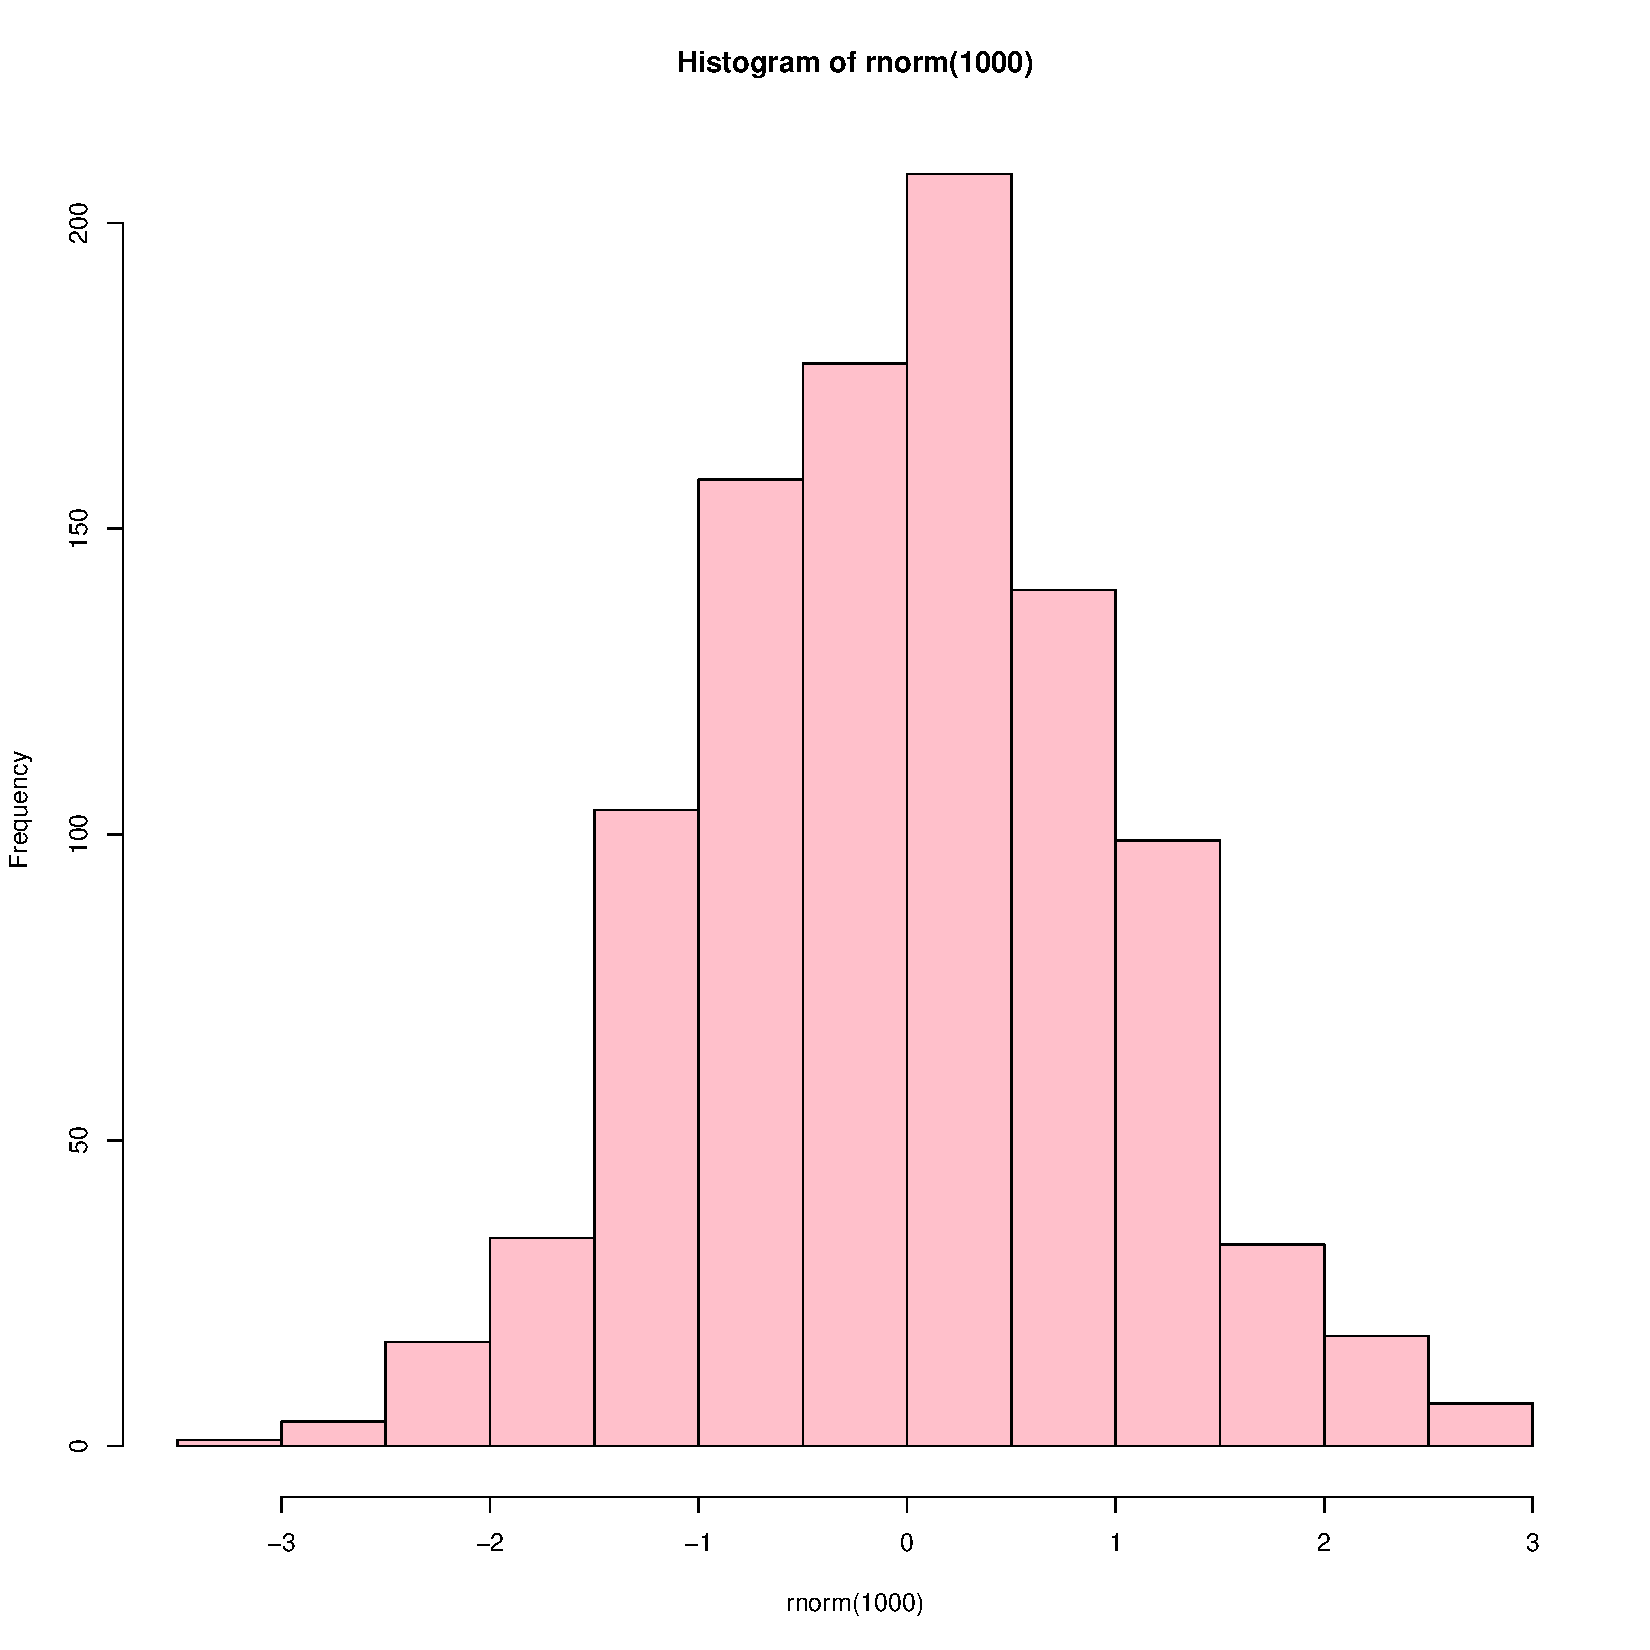
\includegraphics[width=\maxwidth]{figure/HIST-1} 

}



\end{knitrout}
\vspace{0ex}
\end{block}
\vfill

%-- Block 3-2
\vspace{0ex}
\begin{block}{King County Real Estate}
\vspace{0ex}
\begin{knitrout}
\definecolor{shadecolor}{rgb}{0.969, 0.969, 0.969}\color{fgcolor}

{\centering 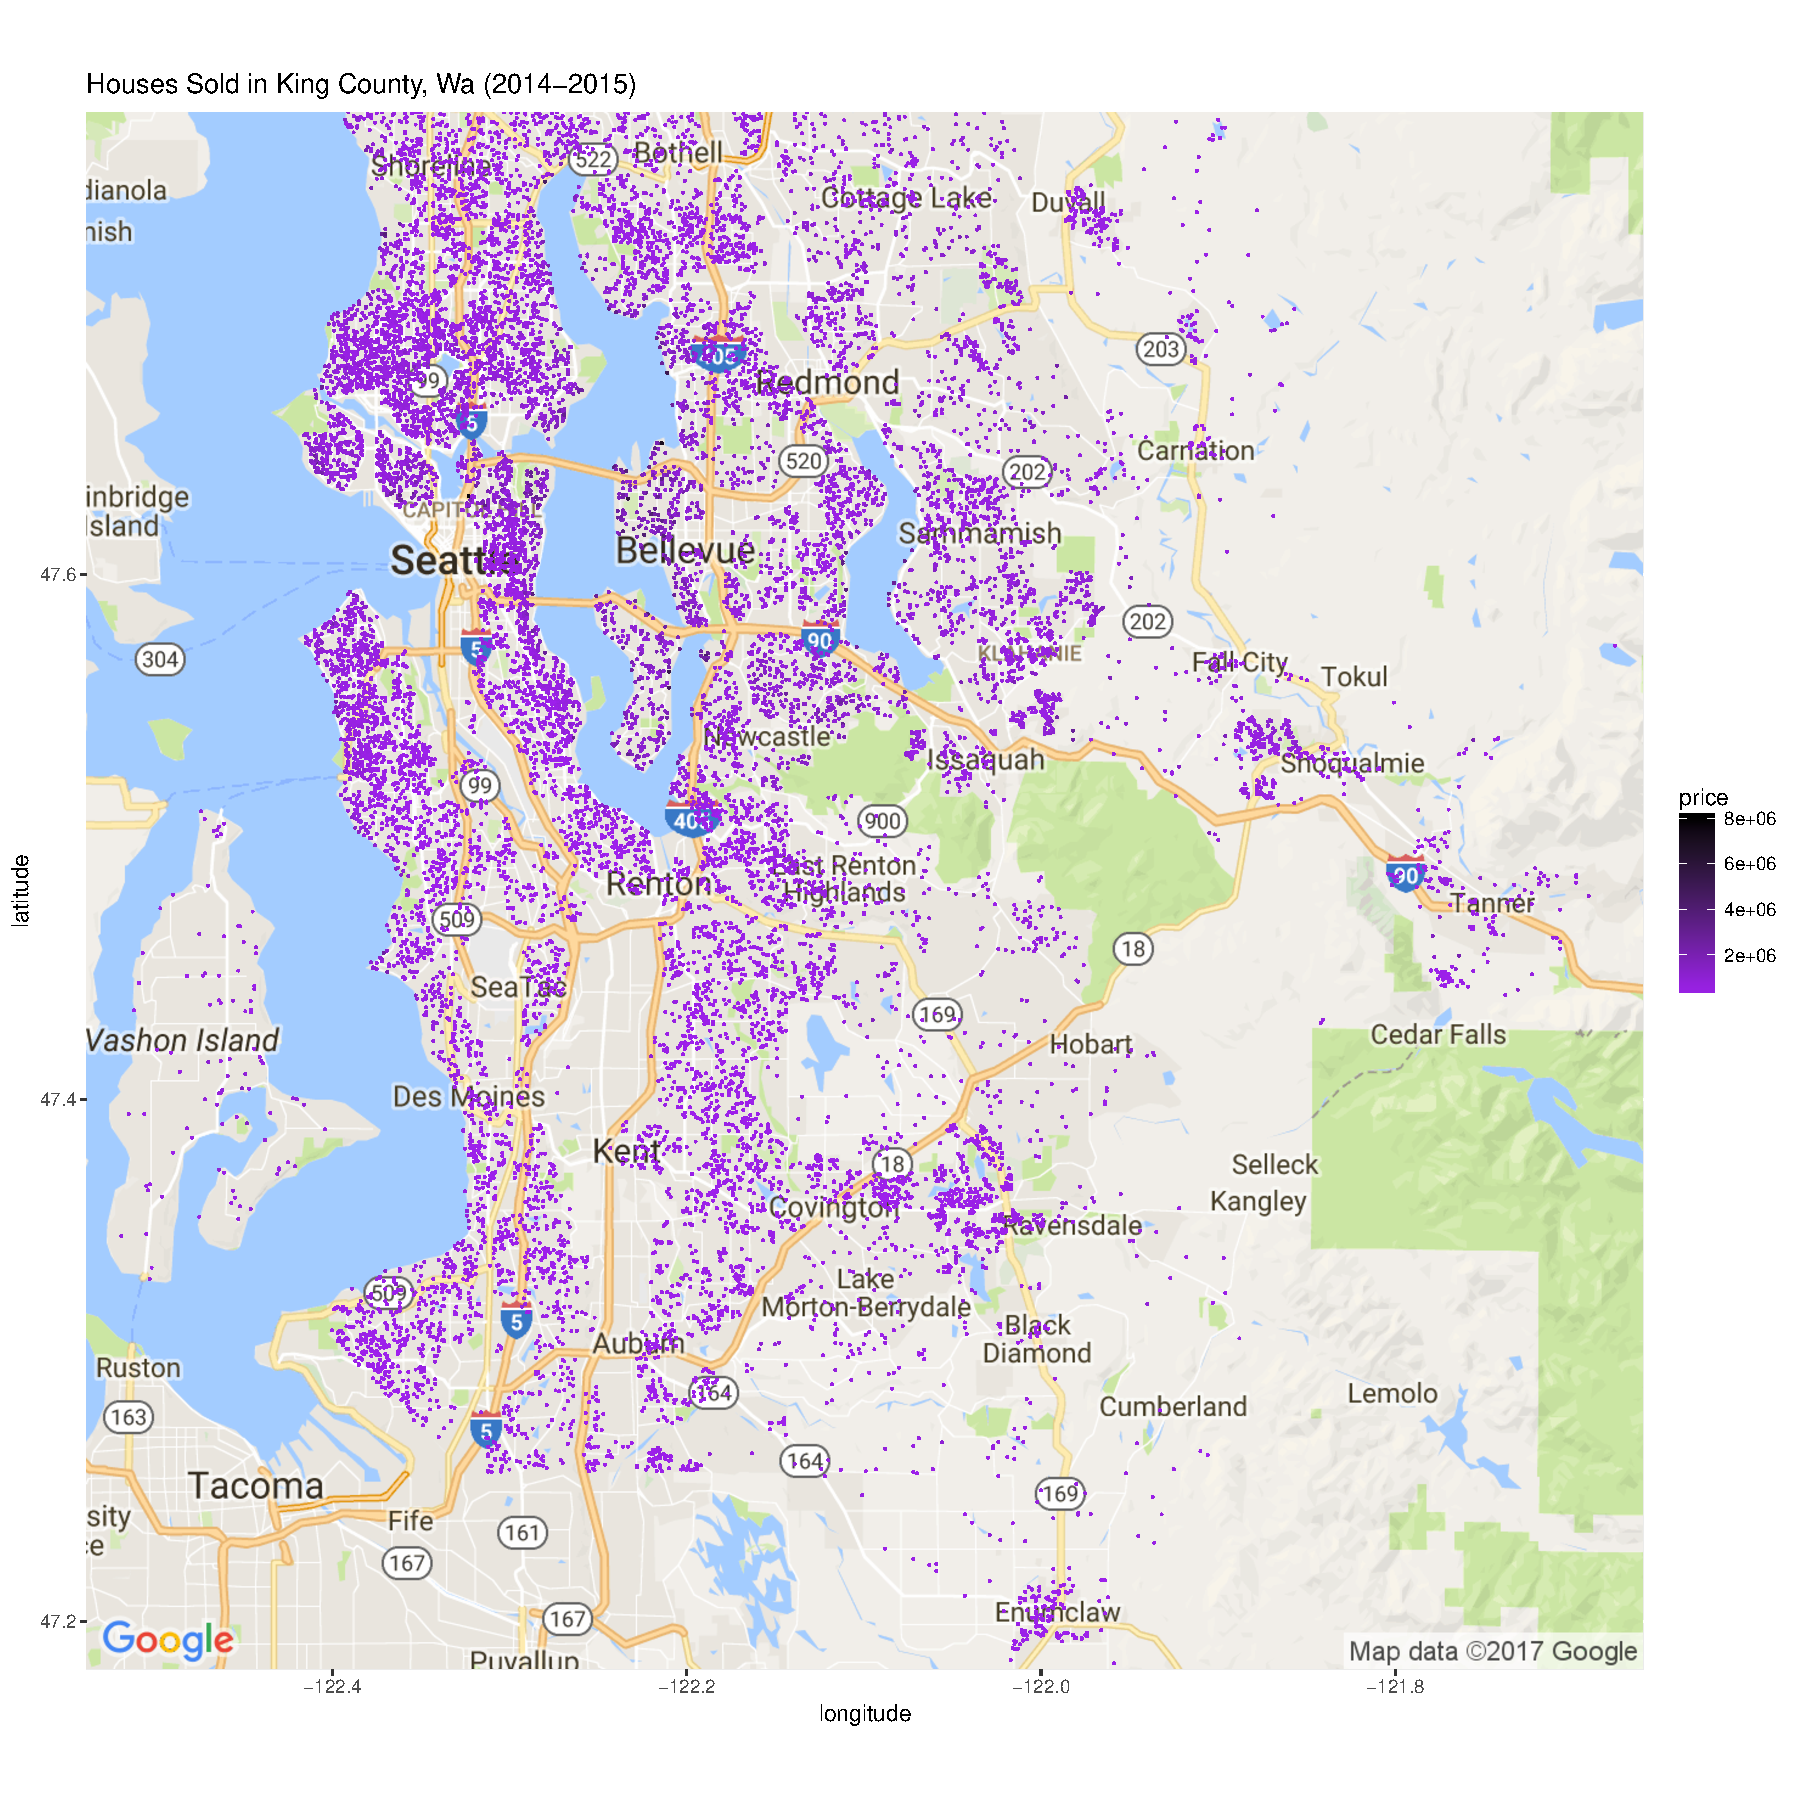
\includegraphics[width=\maxwidth]{figure/KCmap-1} 

}



\end{knitrout}
\vspace{0ex}
\end{block}
\vfill

\end{minipage}
\end{column}%3

%%%%%%%%%%%%%%%%%%%%%%%%%%%%%%%%%%%%%%%%%%%%%%%%%%%%%%%%%%%%%%%%
%-- Column 4 ---------------------------------------------------
\begin{column}{0.23\linewidth}
\begin{minipage}[t][.955\textheight]{\linewidth} 

%-- Block 4-1
\vspace{0ex}
\begin{block}{Random Forest Variable Importance}
\vspace{0ex}
\begin{knitrout}
\definecolor{shadecolor}{rgb}{0.969, 0.969, 0.969}\color{fgcolor}

{\centering 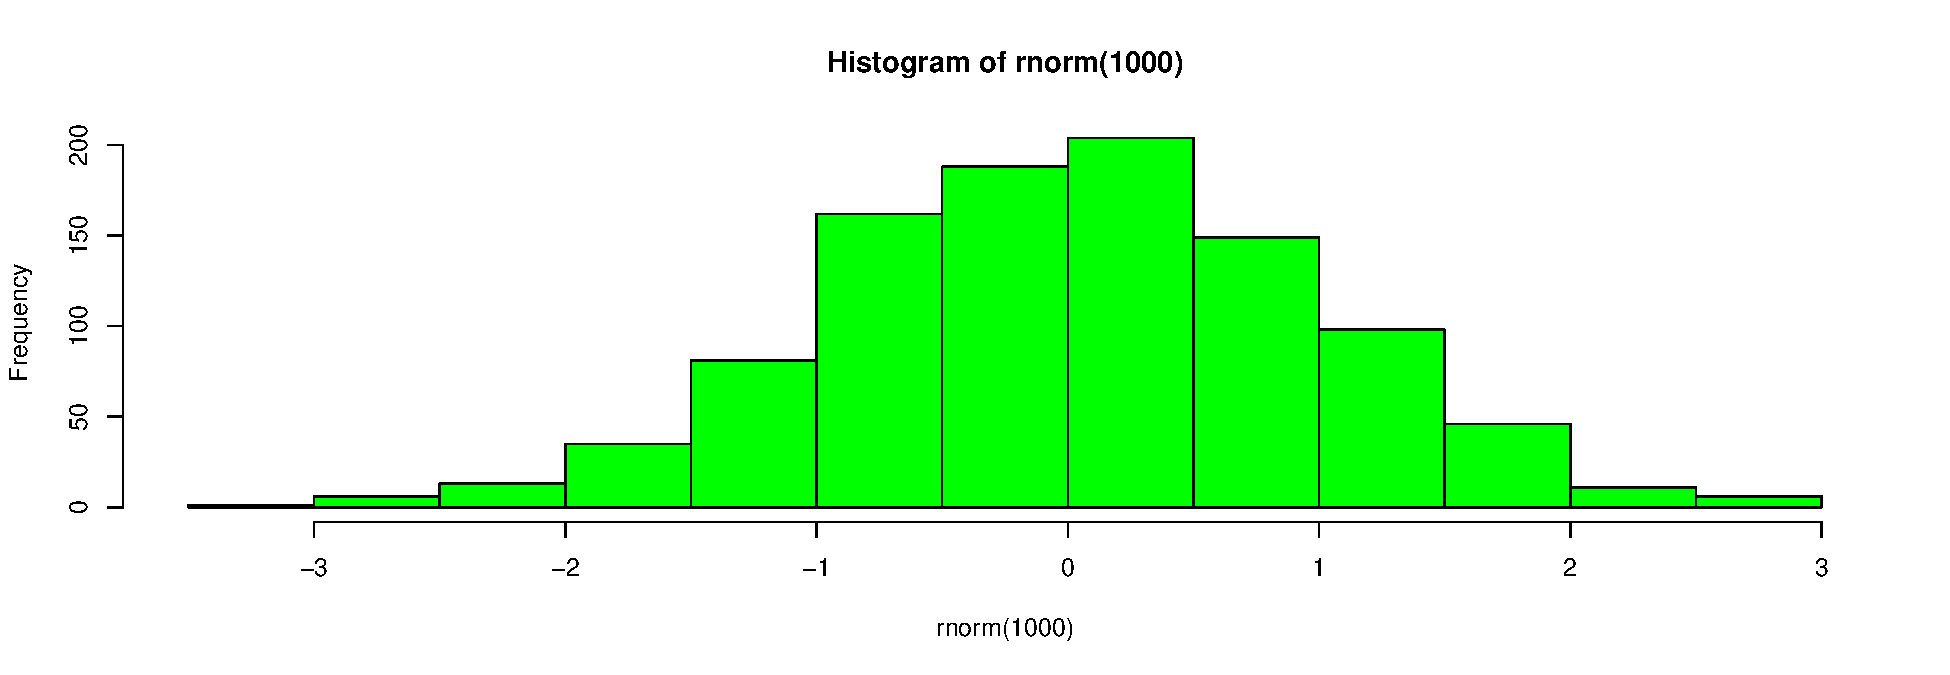
\includegraphics[width=\maxwidth]{figure/HIST2-1} 

}



\end{knitrout}
\vspace{0ex}
\vfill
\end{block}
\vfill

%-- Block 4-2
\begin{block}{Prediction Errors}
\begin{knitrout}
\definecolor{shadecolor}{rgb}{0.969, 0.969, 0.969}\color{fgcolor}

{\centering 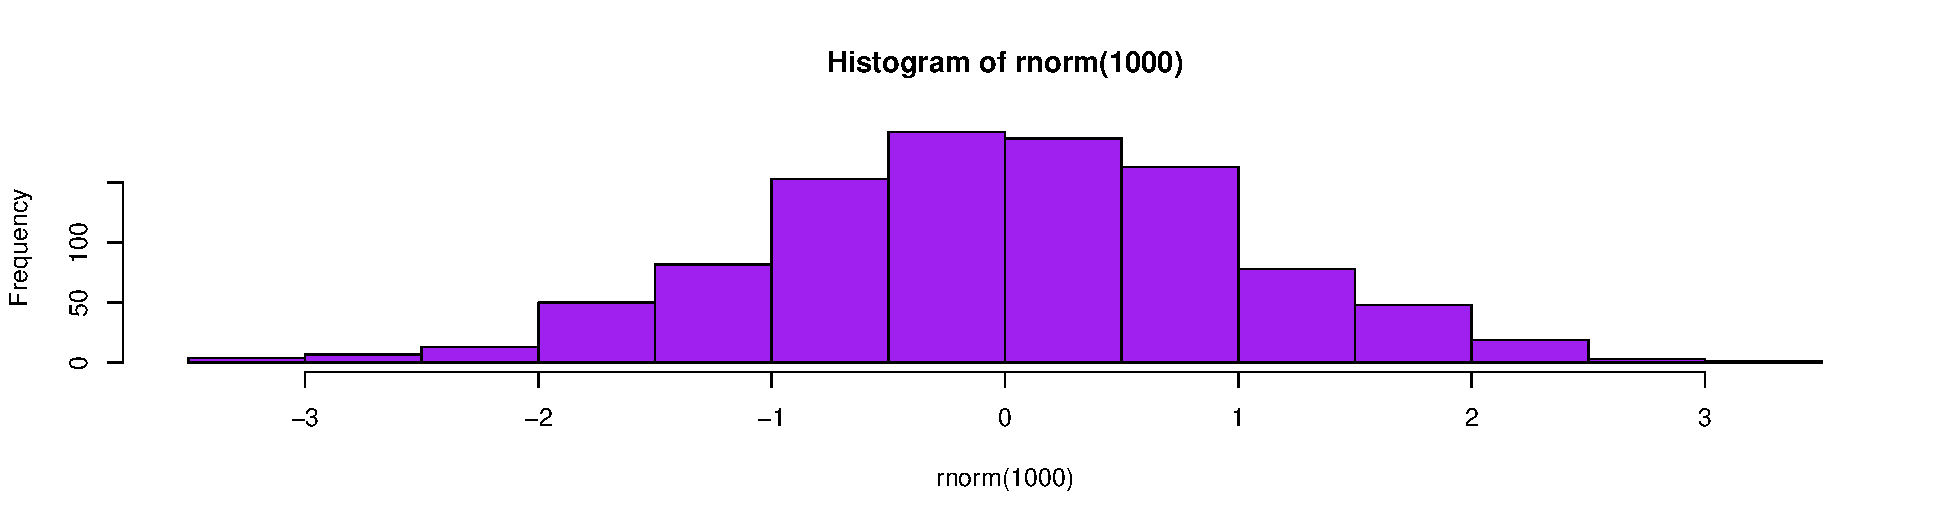
\includegraphics[width=\maxwidth]{figure/HIST3-1} 

}



\end{knitrout}
\vspace{0ex}
\vfill
\end{block}
\vfill

%-- Block 4-3
\begin{block}{Further Directions}
\begin{itemize}
\item Use the models developed in this poster to predict county votes for states that have had similar marriage amendments such as South Carolina, Wisconsin, South Dakota, Florida, Idaho, Alabama, Utah, Michigan, Texas, Arkansas, Louisiana, Kansas, Kentucky, Ohio, and Nebraska. 
\item  Use ensemble methods (combining multiple models) for better prediction.
\item  Make our local maps available via the internet using the shiny server.
\end{itemize}
\vspace{0ex}
\vfill
\end{block}
\vfill

%-- Block 4-4
\begin{block}{References}
\footnotesize
\setbeamertemplate{bibliography item}[text]
\vspace{-1ex}


\bibliographystyle{plain}  % can use plain but comment out natbib at top if using plain
\bibliography{knitr-packages,poster}
\normalsize
\vfill
\end{block} 
\vfill

\end{minipage}
\end{column}%4




\end{columns}
\end{frame}
\end{document}

